%!TeX root = Chapter_Results2
\documentclass[../../CompleteThesis2/Complete_2ndDraft]{subfiles}
%\graphicspath{{../../Figures/}}
\begin{document}

\section[Annual Layer Thickness]{Layer Counting and Annual Layer Thickness}



\section[Diffusion Lengths]{Final Diffusion Length Estimates}

\subsection[AWI B-cores]{AWI B-cores}
\label{Sec:Results_AWIBcores}


%
%
%\begin{figure}[h]
%	\centering
%	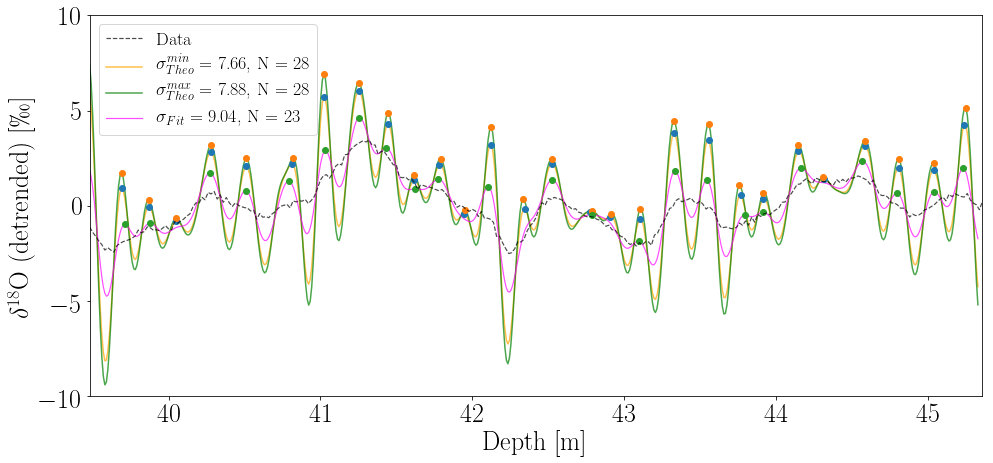
\includegraphics[width=0.8\textwidth]{B23_TheoDiffLens33Theo.png}
%	\caption[]{}
%	\label{fig:B23_BD_Theo}
%\end{figure}
%
%\begin{figure}[h]
%	\centering
%	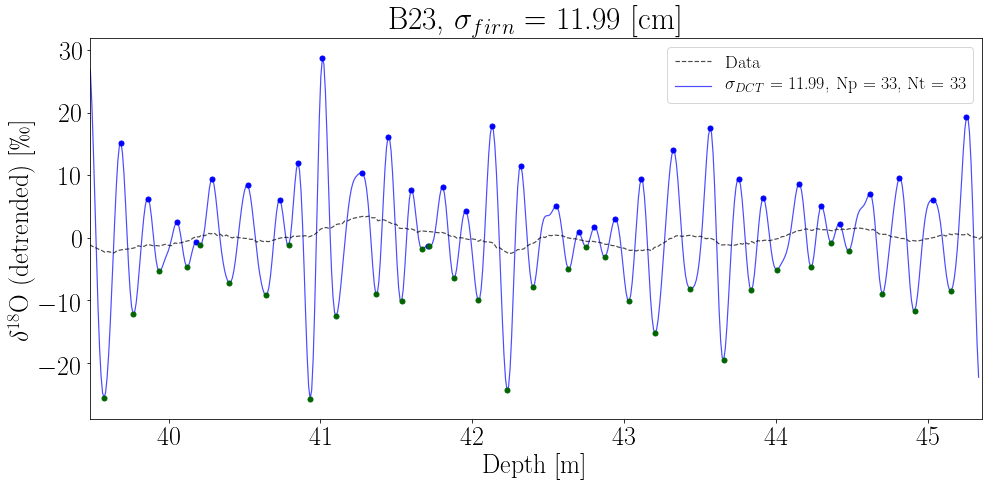
\includegraphics[width=0.8\textwidth]{B23_TheoDiffLens33Opt_only.png}
%	\caption[]{}
%	\label{fig:B23_BD_OptOnly}
%\end{figure}
%
%\begin{figure}[h]
%	\centering
%	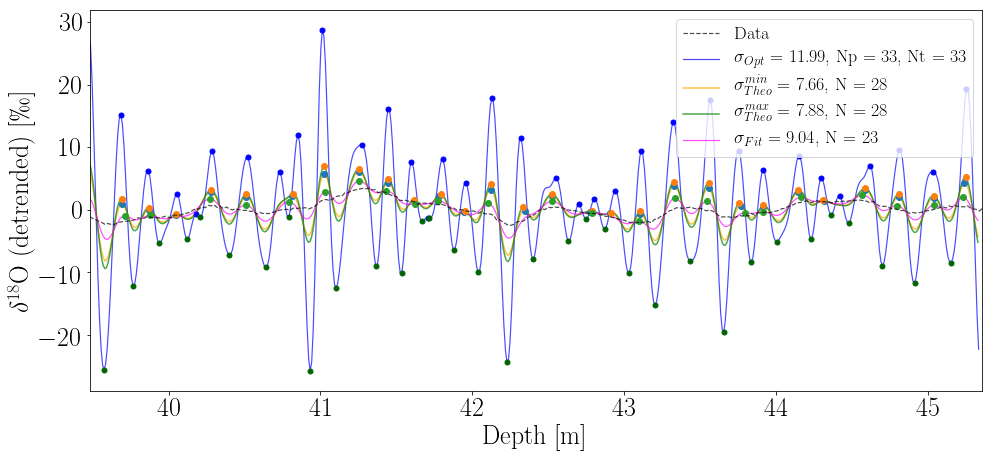
\includegraphics[width=0.8\textwidth]{B23_TheoDiffLens33OptBig.png}
%	\caption[]{}
%	\label{fig:B23_BD_OptBig}
%\end{figure}
%
%
%








\subsection[Alphabet Cores]{Crete and Surrounding Alphabet Cores}
\label{Sec:Results_AlphabetCores}

\begin{table}[ht]
	\centering
	\begin{tabular}{l||*{6}{c | c||}}
		&
		\multicolumn{2}{c}{Crete} & \multicolumn{2}{c}{Site A} & \multicolumn{2}{c}{Site B} & \multicolumn{2}{c}{Site D} & \multicolumn{2}{c}{Site E} & \multicolumn{2}{c||}{Site G} \\
		%\hline
		&
		$\sigma_{\text{opt}}$ & $\sigma_{\text{firn}}$ & $\sigma_{\text{opt}}$ & $\sigma_{\text{firn}}$ & $\sigma_{\text{opt}}$ & $\sigma_{\text{firn}}$ & $\sigma_{\text{opt}}$ & $\sigma_{\text{firn}}$ & $\sigma_{\text{opt}}$ & $\sigma_{\text{firn}}$ & $\sigma_{\text{opt}}$ & $\sigma_{\text{firn}}$ \\
		
		\hline
		FFT & & & & & & & & & & & & \\ 
		DCT & & & & & & & & & & & & \\ 
		NDCT & & & & & & & & & & & & \\ 
	\end{tabular}
\end{table}

\begin{table}[ht]
	\centering
	\begin{tabular}{l||*{6}{c | c||}}
		&
		\multicolumn{2}{c}{Crete} & \multicolumn{2}{c}{Site A} & \multicolumn{2}{c}{Site B} & \multicolumn{2}{c}{Site D} & \multicolumn{2}{c}{Site E} & \multicolumn{2}{c||}{Site G} \\
		%\hline
		&
		$\sigma_{\text{opt}}$ & $\sigma_{\text{firn}}$ & $\sigma_{\text{opt}}$ & $\sigma_{\text{firn}}$ & $\sigma_{\text{opt}}$ & $\sigma_{\text{firn}}$ & $\sigma_{\text{opt}}$ & $\sigma_{\text{firn}}$ & $\sigma_{\text{opt}}$ & $\sigma_{\text{firn}}$ & $\sigma_{\text{opt}}$ & $\sigma_{\text{firn}}$ \\
		
		\hline
		$\sigma_{\text{constant}}$ & & & & & & & & & & & & \\ 
		$\sigma(z)$ & & & & & & & & & & & & \\ 
	\end{tabular}
\end{table}

%\begin{figure}
%	\centering
%	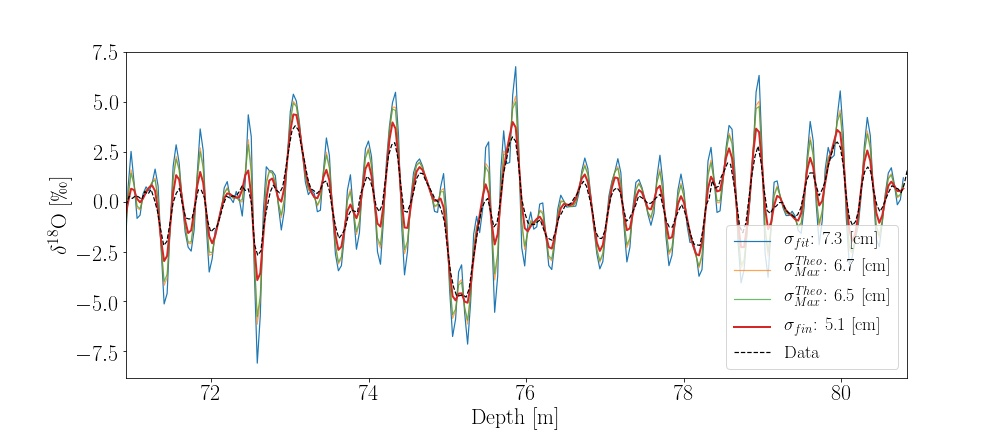
\includegraphics[width=\textwidth]{SiteA_BackDiffused_AllSigmaEst.jpg}
%	\caption[All diffusion length estimate deconvolutions, Site A]{Estimated back diffused data series with different diffusion length estimates: diffusion length estimate from spectral fit ($\sigma_{fit}$), maximum ($\sigma_{Max}^{Theo}$) and minimum ($\sigma_{Min}^{Theo}$) theoretically estimated diffusion lengths and final estimated diffusion length.}
%	\label{fig:SiteA_BackDiffused_AllSigmaEst}
%\end{figure}

\begin{table}[ht]
	\centering
	\begin{tabular}{l||*{6}{c | c||}}
		&
		\multicolumn{2}{c}{Crete} & \multicolumn{2}{c}{Site A} & \multicolumn{2}{c}{Site B} & \multicolumn{2}{c}{Site D} & \multicolumn{2}{c}{Site E} & \multicolumn{2}{c||}{Site G} \\
		%\hline
		&
		$\sigma_{\text{opt}}$ & $\sigma_{\text{firn}}$ & $\sigma_{\text{opt}}$ & $\sigma_{\text{firn}}$ & $\sigma_{\text{opt}}$ & $\sigma_{\text{firn}}$ & $\sigma_{\text{opt}}$ & $\sigma_{\text{firn}}$ & $\sigma_{\text{opt}}$ & $\sigma_{\text{firn}}$ & $\sigma_{\text{opt}}$ & $\sigma_{\text{firn}}$ \\
		
		\hline
		No constraints & & & & & & & & & & & & \\ 
		Constraints & & & & & & & & & & & & \\ 
	\end{tabular}
\end{table}

\section[Temperature Estimates from Data]{Final Temperature Estimates from Optimal Estimated $\sigma$}
\label{Sec:Results_TempEstData}
\todo{RES-DATAEST: Write entire section.}

\subsection[Steady State Solution]{Steady State Solution}
\label{Sec:Results_TempEstData_StSt}
\todo{RES-DATAESTSTST: Write entire section.}

\subsubsection[Accumulation Distributions]{Accumulation Distributions}
\label{Sec:Results_TempEstData_StSt_AccumDists}
\todo{RES-DATAESTACCUM: Write entire section.}

\subsection[Iso-CFM Possibilities]{Further Possibilities of the Iso-CFM}
\label{Sec:Results_TempEstData_IsoCFMPossibilities}
\todo{RES-DATAESTCFM: Write entire section.}

\end{document}
